% section
\section{Image Prediction Architectures} \label{section::related}
 This section will describe a range of state-of-the-art architectures for image prediction. Image prediction is a very broad field, but almost all state-of-the-art solutions
 for image prediction share one common part, the recurrent module. LSTM's are the most used modules in image prediction, as they are able to store information over a long period of time, despite
 the standard RNN (recurrent neural network). All algorithms described here have a different way to perform image prediction, but all use a type of LSTM to store the time-series information.
 
 % subsection
 \subsection{LSTM Autoencoder} \label{subsection::lstm_autoencoder}
  The paper \glqq Unsupervised Learning of Video Representations using LSTMs\grqq by Srivastava et. al. \cite{Srivastava2015} is using the standard LSTM~\ref{subsection::lstm} in an autoencoder 
  architecture for reconstruction and prediction.
  As this thesis topic is image prediction for future images, I will not cover the reconstruction architecture. The architecture is often used as a baseline in newer and more advanced architectures, 
  because it consists of the standard LSTM. The model is typically trained using reconstruction error.
  \begin{figure}[H]
   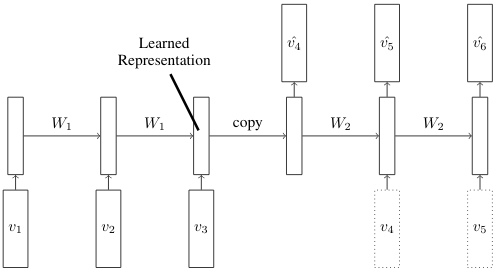
\includegraphics[width=0.45\textwidth]{../Images/srivastava.png}
   \centering
   \caption{Future image prediction model \citep{Srivastava2015}}
   \label{fig:lstm_architecture}
  \end{figure}

 % subsection
 \subsection{ConvLSTM Autoencoder} \label{subsection::convlstm_autoencoder}
  The paper \glqq Convolutional LSTM Network: A Machine Learning Approach for Precipitation Nowcasting\grqq by Shi et. al. \citep{Shi2015} is using a similar architecture as Srivastava et. al. in
  section~\ref{fig:lstm_architecture}, but instead of using the standard LSTM, they use a ConvLSTM~\ref{subsection::convlstm}. This architecture outperforms the Srivastava et. al., because it \glqq 
  captures spatiotemporal correlations better\grqq.
  \begin{figure}[H]
   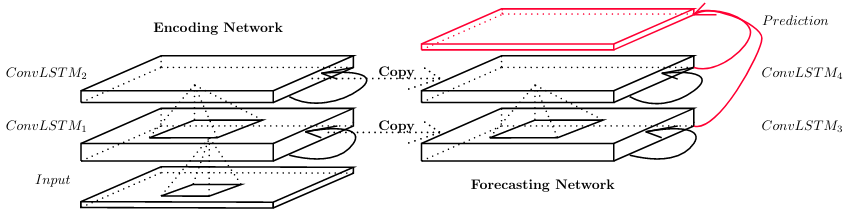
\includegraphics[width=0.65\textwidth]{../Images/shi.png}
   \centering
   \caption{Future image prediction model \citep{Shi2015}}
   \label{fig:lstm_architecture}
  \end{figure}
 
 % subsection
 \subsection{Spatio-temporal Video Autoencoder}
 
 % subsection
 \subsection{PredNet}
  The chosen implementation for the experiments~\ref{section::experiments}.
